% Тип документа
\documentclass[a4paper,12pt]{extarticle}

% Шрифты, кодировки, символьные таблицы, переносы
\usepackage{cmap}
\usepackage[T2A]{fontenc}
\usepackage[utf8x]{inputenc}
\usepackage[russian]{babel}

% Это пакет -- хитрый пакет, он нужен но не нужен
\usepackage[mode=buildnew]{standalone}

\usepackage
	{
		% Дополнения Американского математического общества (AMS)
		amssymb,
		amsfonts,
		amsmath,
		amsthm,
		physics,
		% misccorr,
		% 
		% Графики и рисунки
		wrapfig,
		graphicx,
		subcaption,
		float,
		tikz,
		tikz-3dplot,
		caption,
		csvsimple,
		color,
		booktabs,
		pgfplots,
		pgfplotstable,
		geometry,
		% 
		% Таблицы, списки
		makecell,
		multirow,
		indentfirst,
		%
		% Интегралы и прочие обозначения
		ulem,
		esint,
		esdiff,
		% 
		% Колонтитулы
		fancyhdr,
	}  

\usepackage{xcolor}
\usepackage{hyperref}

 % Цвета для гиперссылок
\definecolor{linkcolor}{HTML}{000000} % цвет ссылок
\definecolor{urlcolor}{HTML}{799B03} % цвет гиперссылок
 
\hypersetup{pdfstartview=FitH,  linkcolor=linkcolor,urlcolor=urlcolor, colorlinks=true}
% Обводка текста в TikZ
\usepackage[outline]{contour}

% Увеличенный межстрочный интервал, французские пробелы
\linespread{1.1} 
\frenchspacing 

 
\usetikzlibrary
	{
		decorations.pathreplacing,
		decorations.pathmorphing,
		patterns,
		calc,
		scopes,
		arrows,
		fadings,
		through,
		shapes.misc,
		arrows.meta,
		3d,
		quotes,
		angles,
		babel
	}


\tikzset{
	force/.style=	{
		>=latex,
		draw=blue,
		fill=blue,
				 	}, 
	%				 	
	axis/.style=	{
		densely dashed,
		blue,
		line width=1pt,
		font=\small,
					},
	%
	th/.style=	{
		line width=1pt},
	%
	acceleration/.style={
		>=open triangle 60,
		draw=magenta,
		fill=magenta,
					},
	%
	inforce/.style=	{
		force,
		double equal sign distance=2pt,
					},
	%
	interface/.style={
		pattern = north east lines, 
		draw    = none, 
		pattern color=gray!60,
					},
	cross/.style=	{
		cross out, 
		draw=black, 
		minimum size=2*(#1-\pgflinewidth), 
		inner sep=0pt, outer sep=0pt,
					},
	%
	cargo/.style=	{
		rectangle, 
		fill=black!70, 
		inner sep=2.5mm,
					},
	%
	caption/.style= {
		midway,
		fill=white!20, 
		opacity=0.9
					},
	%
	}

\newenvironment{tikzpict}
    {
	    \begin{figure}[htbp]
		\centering
		\begin{tikzpicture}
    }
    { 
		\end{tikzpicture}
		% \caption{caption}
		% \label{fig:label}
		\end{figure}
    }


\newcommand{\vbLabel}[3]{\draw ($(#1,#2)+(0,5pt)$) -- ($(#1,#2)-(0,5pt)$) node[below]{#3}}
\newcommand{\vaLabel}[3]{\draw ($(#1,#2)+(0,5pt)$) node[above]{#3} -- ($(#1,#2)-(0,5pt)$) }

\newcommand{\hrLabel}[3]{\draw ($(#1,#2)+(5pt,0)$) -- ($(#1,#2)-(5pt,0)$) node[right, xshift=1em]{#3}}
\newcommand{\hlLabel}[3]{\draw ($(#1,#2)+(5pt,0)$) node[left, xshift=-1em]{#3} -- ($(#1,#2)-(5pt,0)$) }



\newcommand\zi{^{\,*}_i}
\newcommand\sumn{\sum_{i=1}^{N}}

\tikzset{
	coordsys/.style={scale=1.8,x={(1.1cm,-0cm)},y={(0.5cm,1cm)}, z={(0cm,0.8cm)}},
	coordsys/.style={scale=1.5,x={(0cm,0cm)},y={(1cm,0cm)}, z={(0cm,1cm)}}, 
	coordsys/.style={scale=1.5,x={(1cm,0cm)},y={(0cm,1cm)}, z={(0cm,0cm)}}, 
}

\usepgfplotslibrary{units}


% Draw line annotation
% Input:
%   #1 Line offset (optional)
%   #2 Line angle
%   #3 Line length
%   #5 Line label
% Example:
%   \lineann[1]{30}{2}{$L_1$}

\newcommand{\lineann}[4][0.5]{%
    \begin{scope}[rotate=#2, blue,inner sep=2pt, ]
        \draw[dashed, blue!40] (0,0) -- +(0,#1)
            node [coordinate, near end] (a) {};
        \draw[dashed, blue!40] (#3,0) -- +(0,#1)
            node [coordinate, near end] (b) {};
        \draw[|<->|] (a) -- node[fill=white, scale=0.8] {#4} (b);
    \end{scope}
}

\newcommand{\lineannn}[4][0.5]{%
    \begin{scope}[rotate=#2, blue,inner sep=2pt, ]
        \draw[dashed, blue!40] (0,0) -- +(0,#1)
            node [coordinate, near end] (a) {};
        \draw[dashed, blue!40] (#3,0) -- +(0,#1)
            node [coordinate, near end] (b) {};
        % \draw[color=white, color=blue] (a) -- node[fill=white, scale=0.8] {#4} (b);
        \draw[->|] (a)++(-0.3,0) -- (a);
        \draw[->|] (b)++(0.3,0) coordinate (xx) -- (b);
        \draw (xx) node[fill=white, scale=0.8, right] {#4};
    \end{scope}
}

% Круговая стрелка относительно центра (дуга из центра)
\tikzset{
  pics/carc/.style args={#1:#2:#3}{
    code={
      \draw[pic actions] (#1:#3) arc(#1:#2:#3);
    }
  },
  dash/.style={
  	dash pattern=on 5mm off 5mm
  }
}

% Среднее <#1>
\newcommand{\mean}[1]{\langle#1\rangle}

\pgfplotsset{
    % most recent feature set of pgfplots
    compat=newest,
}

% const прямым шрифтом
\newcommand\ct[1]{\text{\rmfamily\upshape #1}}
\newcommand*{\const}{\ct{const}}


\usepackage[europeanresistors,americaninductors]{circuitikz}

% Style to select only points from #1 to #2 (inclusive)
\pgfplotsset{select/.style 2 args={
    x filter/.code={
        \ifnum\coordindex<#1\def\pgfmathresult{}\fi
        \ifnum\coordindex>#2\def\pgfmathresult{}\fi
    }
}}


\usepackage{array}
\usepackage{pstool}


%%%%%%%%%%%%%%%%%%%%%%%%%%%%%%%%%%%%%%%%%%%%%%%%%
\makeatletter
\newif\if@gather@prefix 
\preto\place@tag@gather{% 
  \if@gather@prefix\iftagsleft@ 
    \kern-\gdisplaywidth@ 
    \rlap{\gather@prefix}% 
    \kern\gdisplaywidth@ 
  \fi\fi 
} 
\appto\place@tag@gather{% 
  \if@gather@prefix\iftagsleft@\else 
    \kern-\displaywidth 
    \rlap{\gather@prefix}% 
    \kern\displaywidth 
  \fi\fi 
  \global\@gather@prefixfalse 
} 
\preto\place@tag{% 
  \if@gather@prefix\iftagsleft@ 
    \kern-\gdisplaywidth@ 
    \rlap{\gather@prefix}% 
    \kern\displaywidth@ 
  \fi\fi 
} 
\appto\place@tag{% 
  \if@gather@prefix\iftagsleft@\else 
    \kern-\displaywidth 
    \rlap{\gather@prefix}% 
    \kern\displaywidth 
  \fi\fi 
  \global\@gather@prefixfalse 
} 
\newcommand*{\beforetext}[1]{% 
  \ifmeasuring@\else
  \gdef\gather@prefix{#1}% 
  \global\@gather@prefixtrue 
  \fi
} 
\makeatother
%%%%%%%%%%%%%%%%%%%%%%%%%%%%%%%%%%%%%%%%%%%%%%%%%

\geometry		
	{
		left			=	2cm,
		right 			=	2cm,
		top 			=	3cm,
		bottom 			=	3cm,
		bindingoffset	=	0cm
	}

%%%%%%%%%%%%%%%%%%%%%%%%%%%%%%%%%%%%%%%%%%%%%%%%%%%%%%%%%%%%%%%%%%%%%%%%%%%%%%%



	%применим колонтитул к стилю страницы
\pagestyle{fancy} 
	%очистим "шапку" страницы
\fancyhead{} 
	%слева сверху на четных и справа на нечетных
\fancyhead[R]{\labauthors} 
	%справа сверху на четных и слева на нечетных
\fancyhead[L]{Отчёт по лабораторной работе №\labnumber} 
	%очистим "подвал" страницы
\fancyfoot{} 
	% номер страницы в нижнем колинтуле в центре
\fancyfoot[C]{\thepage} 

%%%%%%%%%%%%%%%%%%%%%%%%%%%%%%%%%%%%%%%%%%%%%%%%%%%%%%%%%%%%%%%%%%%%%%%%%%%%%%%

\renewcommand{\contentsname}{Оглавление}

\usepackage{tocloft}
% \renewcommand{\cftpartleader}{\cftdotfill{\cftdotsep}} % for parts
% \renewcommand{\cftsectiondotsep}{\cftdotsep}% Chapters should use dots in ToC
\renewcommand{\cftsecleader}{\cftdotfill{\cftdotsep}}
%\renewcommand{\cftsecleader}{\cftdotfill{\cftdotsep}} % for sections, if you really want! (It is default in report and book class (So you may not need it).
% ---------
% \newcommand{\cftchapaftersnum}{.}%
% \usepackage{titlesec}
% \titlelabel{\thetitle.\quad}
\usepackage{secdot}
\sectiondot{subsection}

\begin{document}

\def\labauthors{Карусевич А.А., Шиков А.П.}
\def\labgroup{440}
\def\labnumber{2}
\def\labtheme{Измерение статистических характеристик полевого транзистора}
\renewcommand{\vec}{\mathbf}
\renewcommand{\phi}{\varphi}
\renewcommand{\hat}{\widehat}

\begin{titlepage}

\begin{center}

{\small\textsc{Нижегородский государственный университет имени Н.\,И. Лобачевского}}
\vskip 1pt \hrule \vskip 3pt
{\small\textsc{Радиофизический факультет}}

\vfill

{\Large Отчет по лабораторной работе №\labnumber\vskip 12pt\bfseries \labtheme}
	
\end{center}

\vfill
	
\begin{flushright}
	{Выполнили студенты \labgroup\ группы\\ \labauthors}%\vskip 12pt Принял:\\ Менсов С.\,Н.}
\end{flushright}
	
\vfill
	
\begin{center}
	Нижний Новгород, \the\year
\end{center}

\end{titlepage}



\section{Введение}
Полевыми транзисторами (ПТ) называются полупроводниковые приборы, работа которых основана на управлении размерами токопроводящей области (канала) посредством изменения напряженности поперечного электрического поля. Структура:
\begin{figure}[h!]
	\centering
	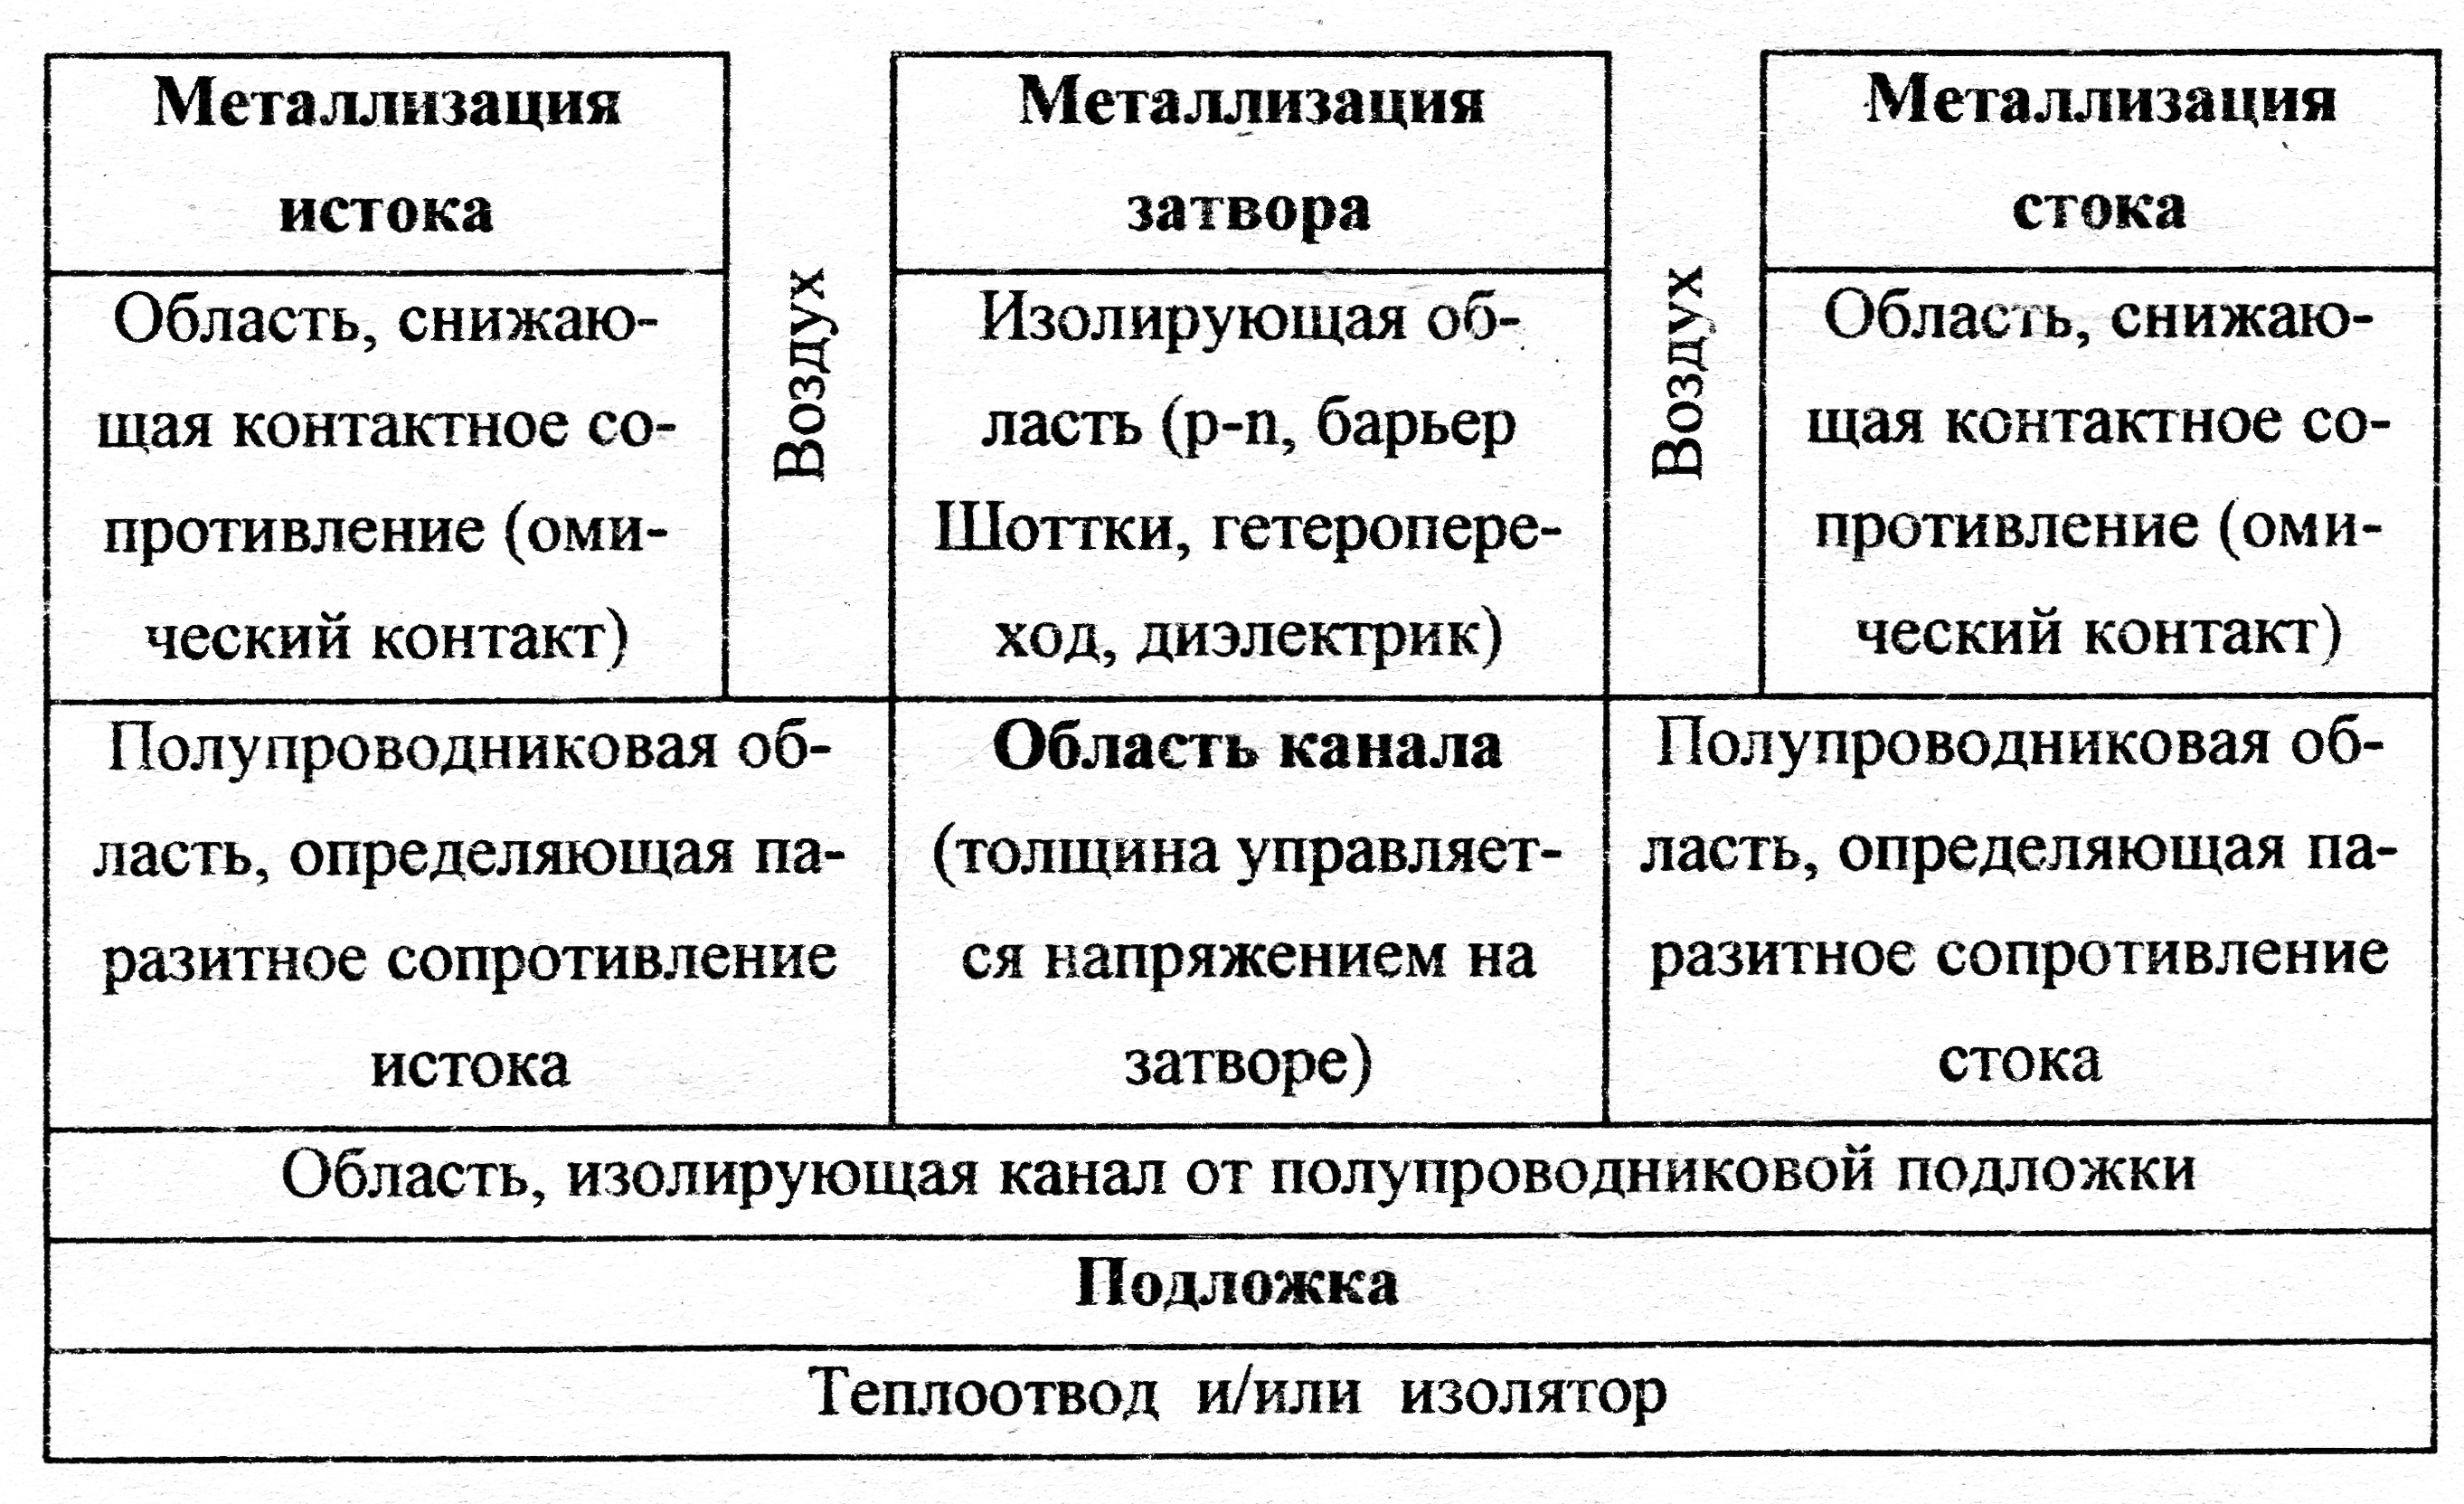
\includegraphics[width=0.5\linewidth]{imgs/fig1.jpg}
	\caption{Структурная схема полевого транзистора}
	\label{fig:1}
\end{figure}

Ток прибора протекает по полупроводниковой области, называемой каналом. В ПТ используется движение носителей заряда только одного знака, поэтому прибор иногда называют униполярным транзистором. Они "истекают" из электрода, называемого истоком, движутся вдоль канала и "стекают" в сток. Затвор транзистора является управляющим электродом. Электрическое поле, возникающее при подаче напряжения между истоком и затвором,Ю изменяет проводимость канала и, следовательно, ток через канал. Таким образом. ток прибора изменяется за счет электрического поля, направленного перпендикулярно движению носителей в канале (поэтому транзистор называют полевым). Носители движутся от истока к стоку под действием продольного электрического поля, создаваемого напряжением между истоком и стоком. Подложка -конструктивный слой полупроводника, который вырезают из полупроводникового слитка, шлифуют и полируют, а затем используют как основу для выращивания на нем тонких эпитаксиальных полупроводниковых слоев, из которых формируется структура приборов.

Существует два основных типа ПТ, различающихся физической структурой и способом управления проводимостью канала. В ПТ с изолированны затвором между металлическим затвором и каналом расположен слой диэлектрика так, что образуется структура металл/диэлектрик/полупроводник. Поэтому такие транзисторы называются МДП-транзисторами. Поперечное электрическое поле, проникая через слой диэлектрика, управляет концентрацией носителей заряда в полупроводниковом канале. Такие транзисторы делятся, в свою очередь на приборы со встроенным и индуцированным каналом. В ПТ с управляющим переходом металлический электрод затвора образует с приповерхностным слоем полупроводника выпрямляющий контакт, на который в рабочем режиме подается обратное напряжение (изоляция затвора путем запирания выпрямляющего контакта). В качестве управляющего перехода могут использоваться p-n переход, гетеропереход или контакт Шоттки.

Все ПТ различают также по типу проводимости канала: транзисторы с каналом p и n-типа. Полярности рабочих напряжений смещения, подаваемых на электроды этих транзисторов, противоположны.

Характерным для всех ПТ является очень малый ток в цепи затвора, так как затвор либо изолирован диэлектриком, либо образует с каналом управляющий переход, включаемый в обратном направлении. Так как затвор в электрических схемах является входным электродом, то ПТ обладает высоким входным сопротивлением на постоянном токе. В этом заключается отличие ПТ от биполярных транзисторов, во входной цепи которых (обычно базовой) протекает значительный ток при прямом напряжении на переходе эмиттер-база. Поэтому входное сопротивление биполярных транзисторов относительно мало. 

В связи с указанным различием входных сопротивлений говорят, что ПТ - это прибор, управляемый напряжением (электрическим полем), а биполярный - управляемый током. В приборах, управляемых напряжением, напряжение на входном электроде из-за высокого входного сопротивления $R_\text{ВХ}$ практически не зависит от параметров самого прибора и определяется ЭДС генератора входного сигнала, если $R_\text{ВХ} \gg R_\text{ГЕН}$, где $R_\text{ГЕН}$ - внутреннее сопротивление генератора. В приборах, управляемых током, входной ток из-за малого входного сопротивления слабо зависит от параметров прибора и определяется током генератора входного сигнала (при $R_\text{ВХ} \ll R_\text{ГЕН}$).

\section{Полевые транзисторы с управляющим переходом}
\subsection{Структура и принцип действия}
В полевых транзисторах с управляющим переходом изменение потока основных носителей происходит с помощью выпрямляющего электрического перехода, смещенного в обратном направлении.

Полевой транзистор с управляющим p-n переходом имеет два омических контакта к области, по которой проходит управляемый ток основных носителей заряда, один управляющий электронно-дырочный переход и один изолирующий от подложки p-n переход. На оба перехода подаются запирающие напряжения
\begin{figure}[h!]
	\centering
	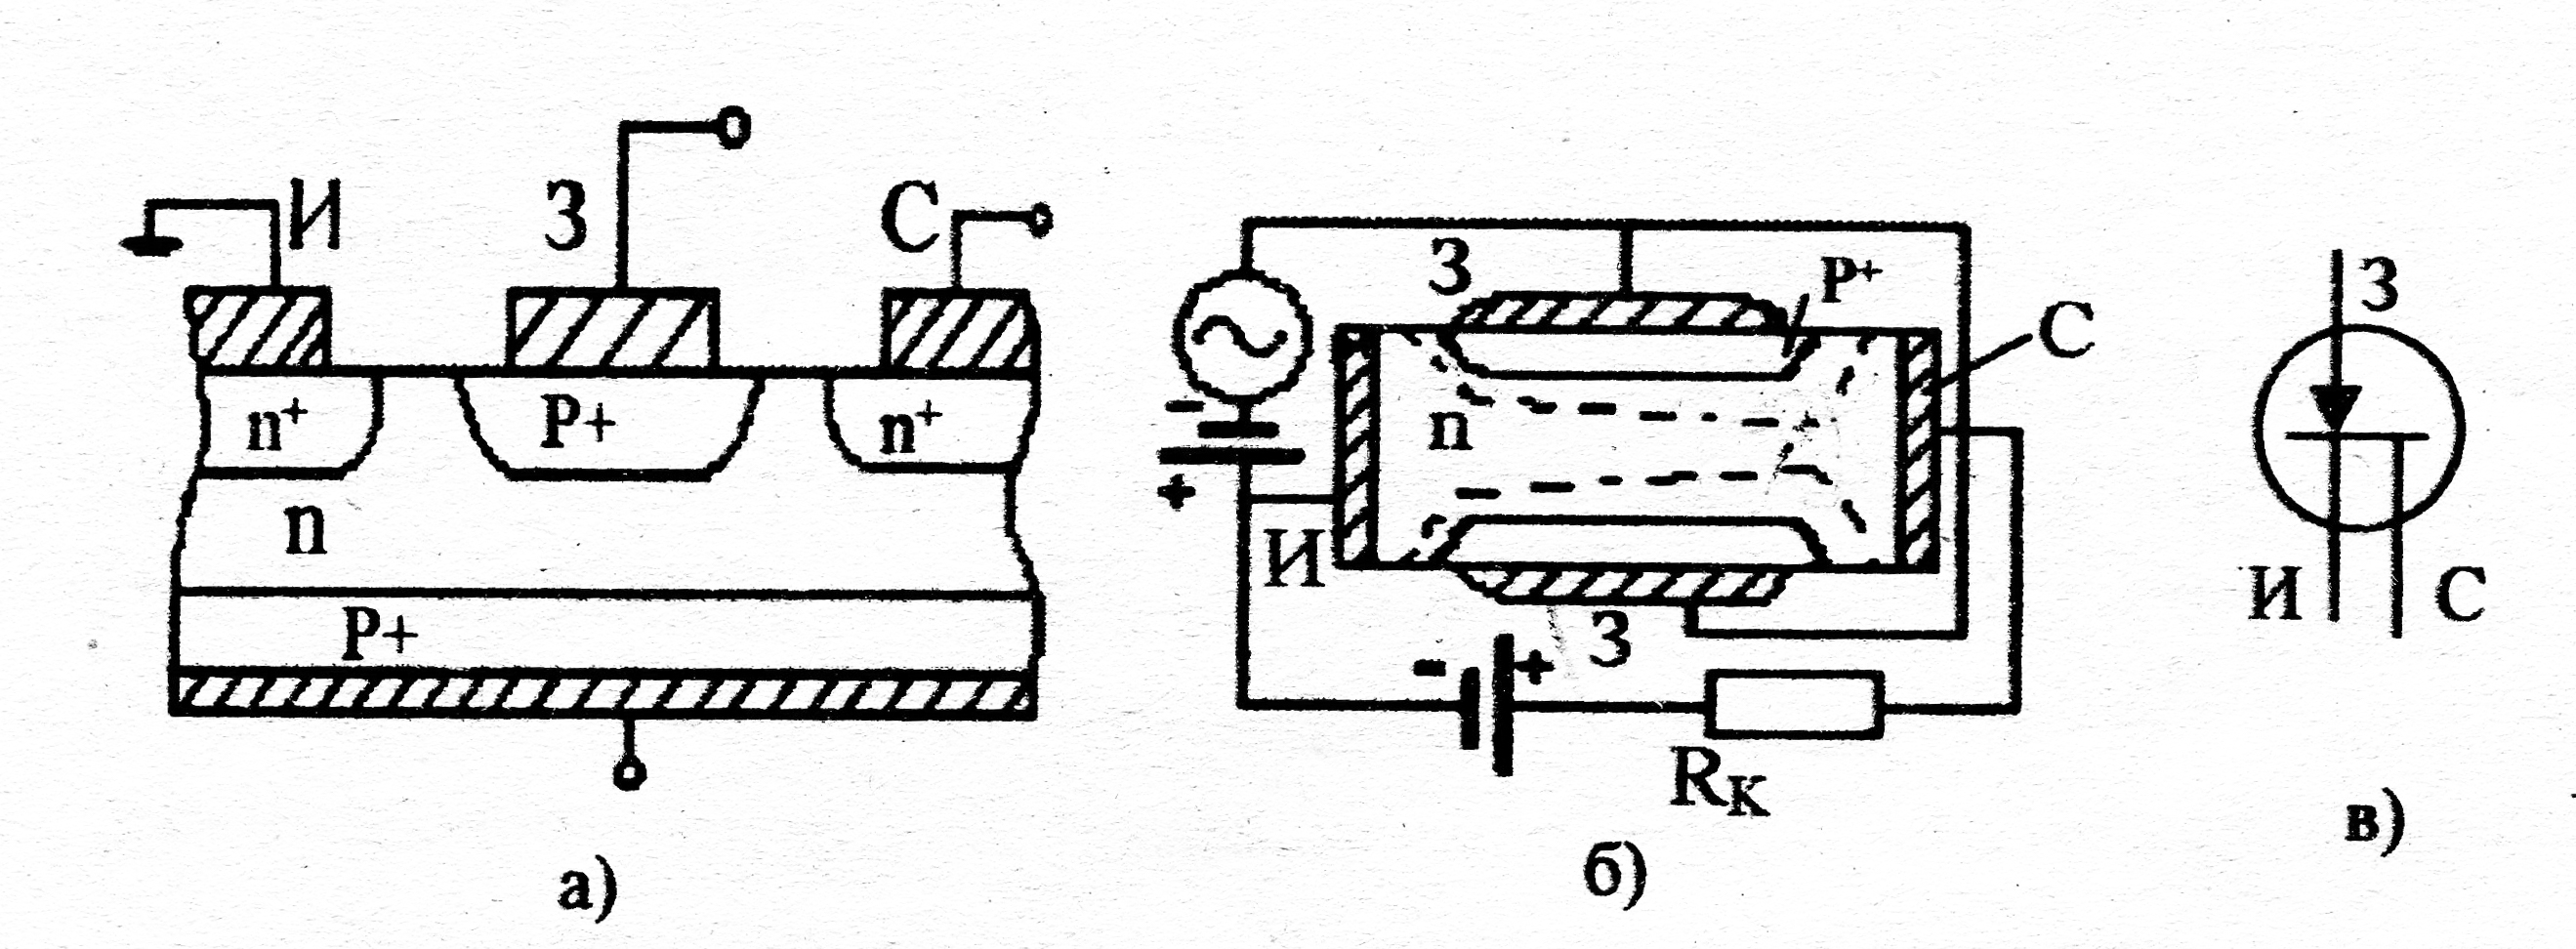
\includegraphics[width=0.5\linewidth]{imgs/fig2.jpg}
	\caption{Полевой транзистор с управляющим p-n переходом: а) реальная структура транзистора; б) схема включения модельной (симметричной) структуры транзистора по схеме с общим истоком; в) графическое обозначение полевого транзистора с управляющим переходом. Обозначения: И-исток; З-затвор; С-сток; n-область канала; $p^+$ - область затвора p-типа (значок "+" обозначает высокий уровень содержания легирующей примеси); пунктиром показана обедненная электронами область p-n переходов затвора в слое канала}
	\label{fig:2}
\end{figure}

Управление током стока происходит при изменении обратного напряжения на p-n переходе затвора. При этом изменяется толщина p-n перехода и, следовательно, толщина канала - области, по которой протекает управляемый ток. В связи с тем, что обратные токи малы, мощность, затрачиваемая для управлении током стока, оказывается также малой. Поэтому полевой транзистор обеспечивает усиление сигнала по мощности, току и напряжению. Принцип действия полевого транзистора аналогичен вакуумному триоду. Исток в полевом транзисторе подобен катоду, затвор - сетке, сток - аноду.

\subsection{Статические характеристики}
Важнейшими семействами статистических характеристик ПТ являются выходные статистические характеристики и характеристики передачи.

Выходные статистические характеристики представляют собой зависимость тока стока $J_C$ от напряжения на стоке относительно истока $U_\text{СИ}$ при различных постоянных напряжениях на затворе $U_\text{ЗИ}: J_C=f(U_\text{СИ})$ при $U_\text{ЗИ} = const$:
\begin{figure}[h!]
	\centering
	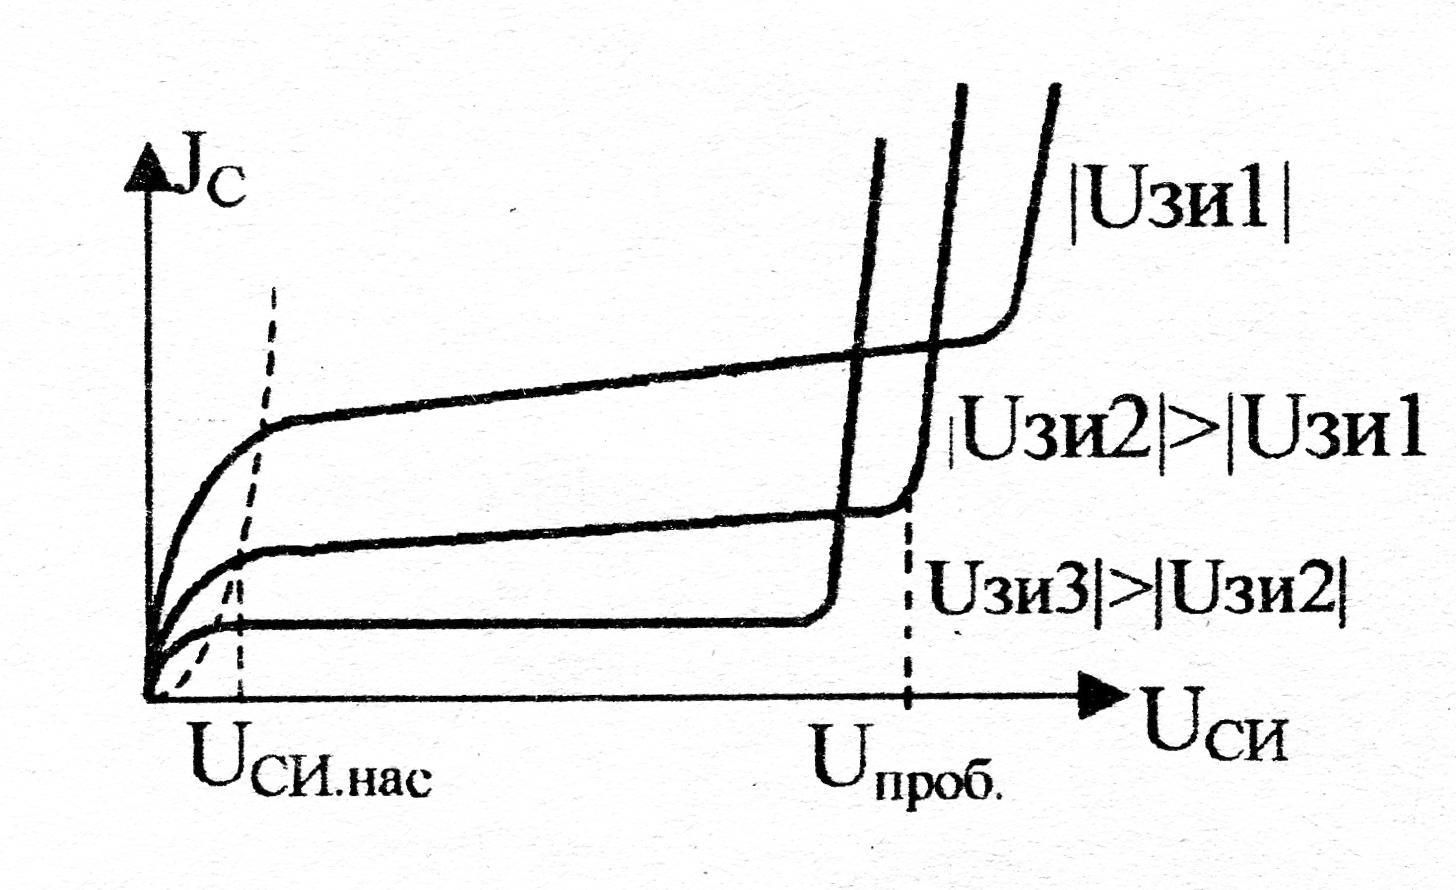
\includegraphics[width=0.5\linewidth]{imgs/fig3.jpg}
	\caption{Выходные статистические ВАХ ПТ при различных напряжениях исток-затвор}
	\label{fig:3}
\end{figure}

На начальном (крутом) участке отличие от линейной зависимости объясняется увеличением толщины управляющего p-n перехода около стока, при котором поперечное сечение канала уменьшается, а сопротивление канала увеличивается. Другая причина нелинейности выходной характеристики - уменьшение подвижности носителей заряда в канале при увеличении в нем напряженности электрического поля.

При $U_\text{СИ} = U_\text{СИ.нас.}$ происходит смыкание ОПЗ затворов сначала около стока. при дальнейшем увеличении $U_\text{СИ}$ длина перекрытой части канала увеличивается, причем статическое сопротивление канала растет пропорционально увеличению напряжения стока, поэтому ток стока остается постоянным (насыщенным).

При увеличении $|U_\text{ЗИ}|$ уменьшается исходное поперечное сечение канала. Поэтому начальные участки выходных характеристик имеют меньший наклон, что соответствует большему начальному статическому сопротивлению канала. Перекрытие канала происходит при меньших напряжениях насыщения.

При некотором напряжении на стоке возникает пробой p-n перехода затвора, обратное напряжение на котором изменяется вдоль канала, достигая максимума у стокового конца. Напряжение, приложенное к p-n переходу затвора в этом месте равно $U_\text{СИ}+|U_\text{ЗИ}|$. Поэтому чем больше $|U_\text{ЗИ}|$, тем меньше $U_\text{СИ.проб.}$

Характеристики передачи представляют собой зависимость $J_C=f(U_\text{ЗИ})$ при $U_\text{СИ} = const$:
\begin{figure}[h!]
	\centering
	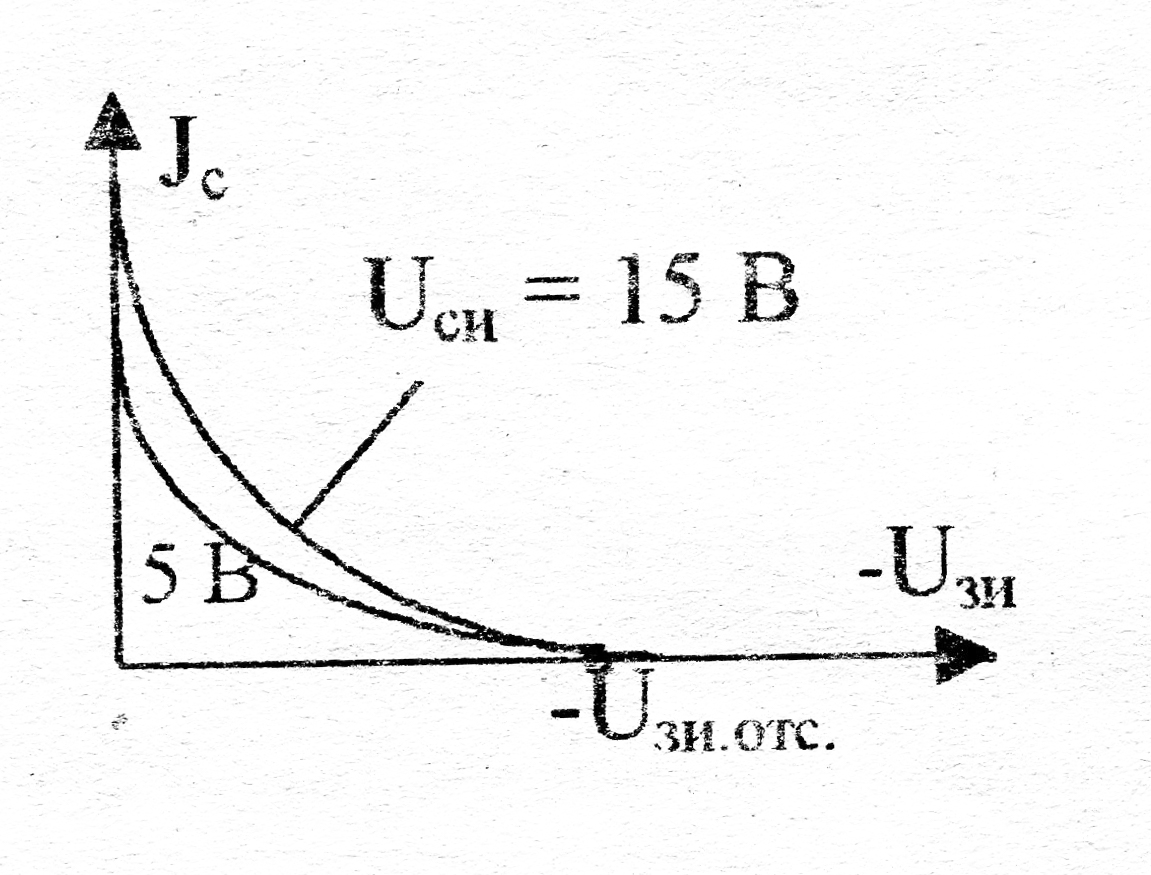
\includegraphics[width=0.5\linewidth]{imgs/fig4.jpg}
	\caption{Статическая передаточная ВАХ}
	\label{fig:4}
\end{figure}

Они снимаются в режиме насыщения тока стока (пологая часть выходных статических характеристик), т.к. это основной
рабочий режим полевого транзистора. При изменении $U_\text{СИ}$ смещением характеристик передачи практически можно
пренебречь. При $U_\text{ЗИ} = U_\text{ЗИ.отс}, J_C=0$

\newpage
\section{Экспериментальная часть}
\subsection{Экспериментальная установка}
В состав установки входят: два источника питания 1, многопредельный миллиамперметр 2, измерительный модуль 3,
осциллограф 4 и генератор сигналов 5. Внешний вид установки и измерительного модуля приведен на рис. \ref{fig:5}. 
\begin{figure}[h!]
	\centering
	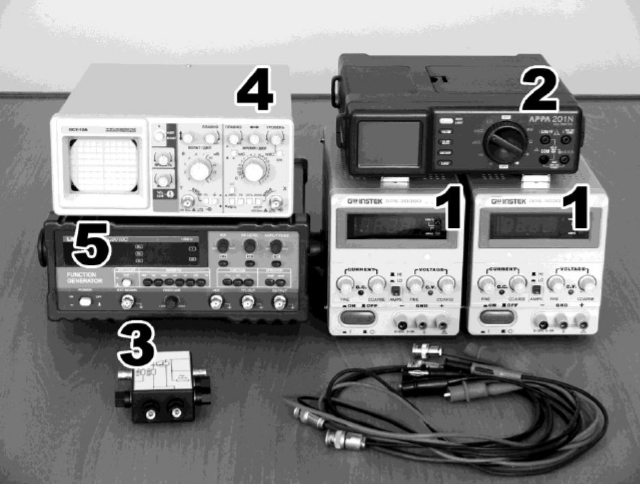
\includegraphics[width=0.4\linewidth]{imgs/setup.png}
	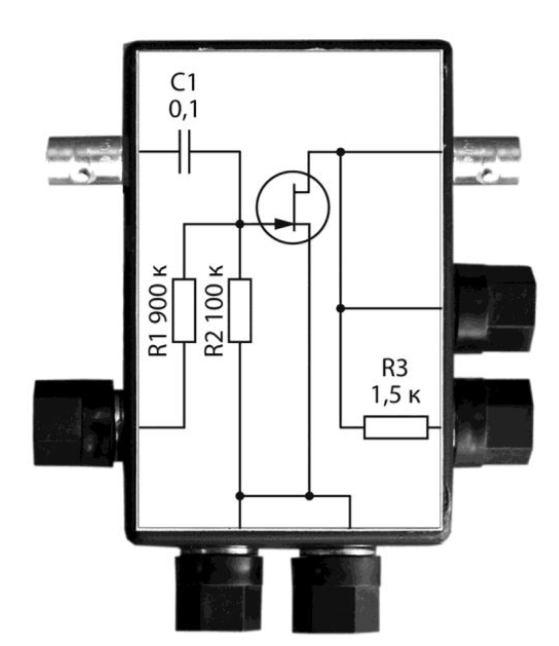
\includegraphics[width=0.3\linewidth]{imgs/scheme.png}
	\caption{Внешний вид установки и измерительного модуля}
	\label{fig:5}
\end{figure}

\subsection{Измерение переходных характеристик транзистора}
Для снятия зависимости $I_c = f(U_{\text{з}})$ измерительный модуль был подключен по схеме \ref{fig:6}.
\begin{figure}[h!]
	\centering
	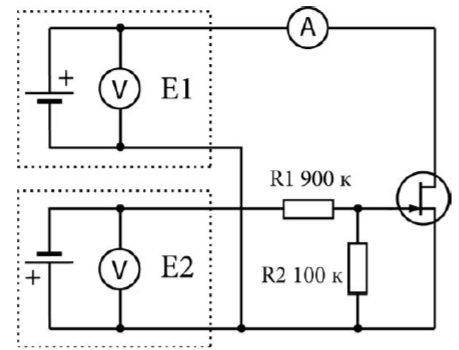
\includegraphics[width=0.35\linewidth]{imgs/ex1.png}
	\caption{Схема подключения для измерения переходных характеристик транзистора}
	\label{fig:6}
\end{figure}

Для значений напряжения на стоке $U_c = 0.5,2,10$ В были сняты переходные характеристики $I_c = f(U_{\text{з}})$(см.
рис. \ref{fig:7}). 
\begin{figure}[h!]
	\centering
	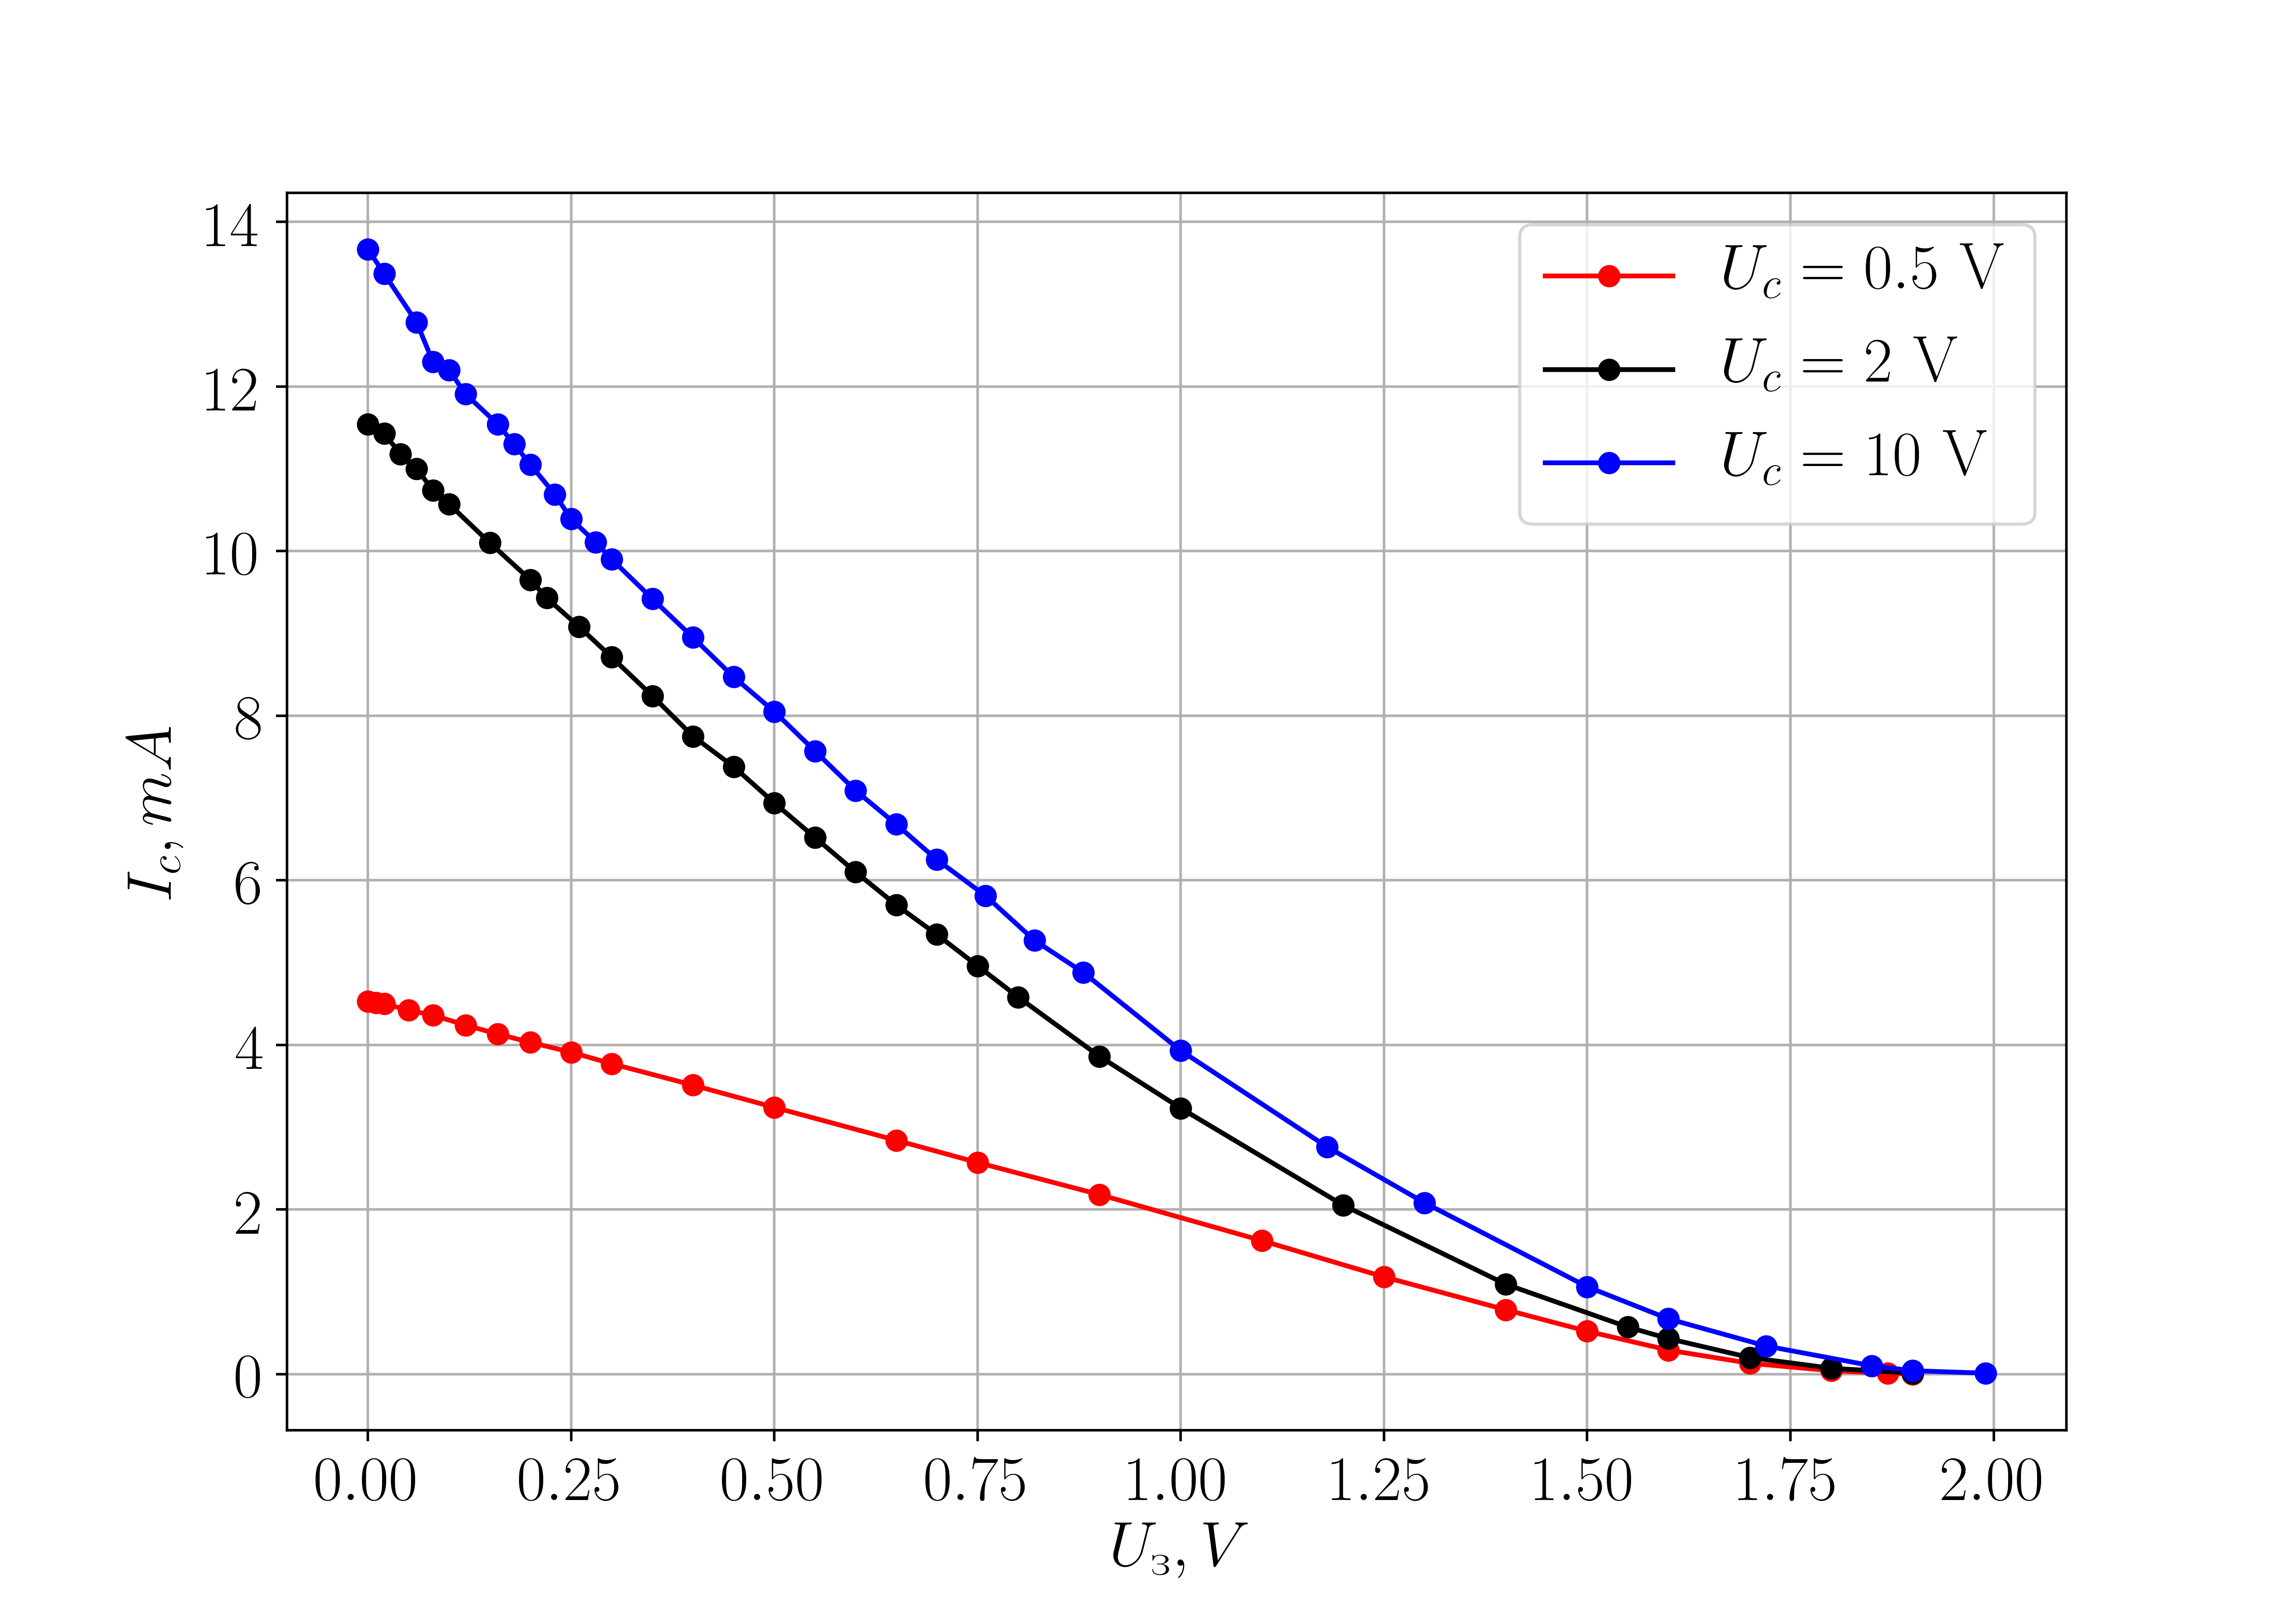
\includegraphics[width=0.7\linewidth]{fig/task1.png}
	\caption{Переходные характеристики транзистора для различных значений $U_c$}
	\label{fig:7}
\end{figure}

Для каждой переходной характеристики была рассчитана крутизна??.

\subsection{Измерение выходных характеристик транзистора}
Не изменяя схему подключения транзистора (см рис. \ref{fig:6}) было проведено измерение семейства выходных характеристик
при напряжении на затворе $U_{\text{з}} = 0,-0.5,-1,-1.5$ В. Результаты приведены на рис.\ref{fig:8}

\begin{figure}[h!]
	\centering
	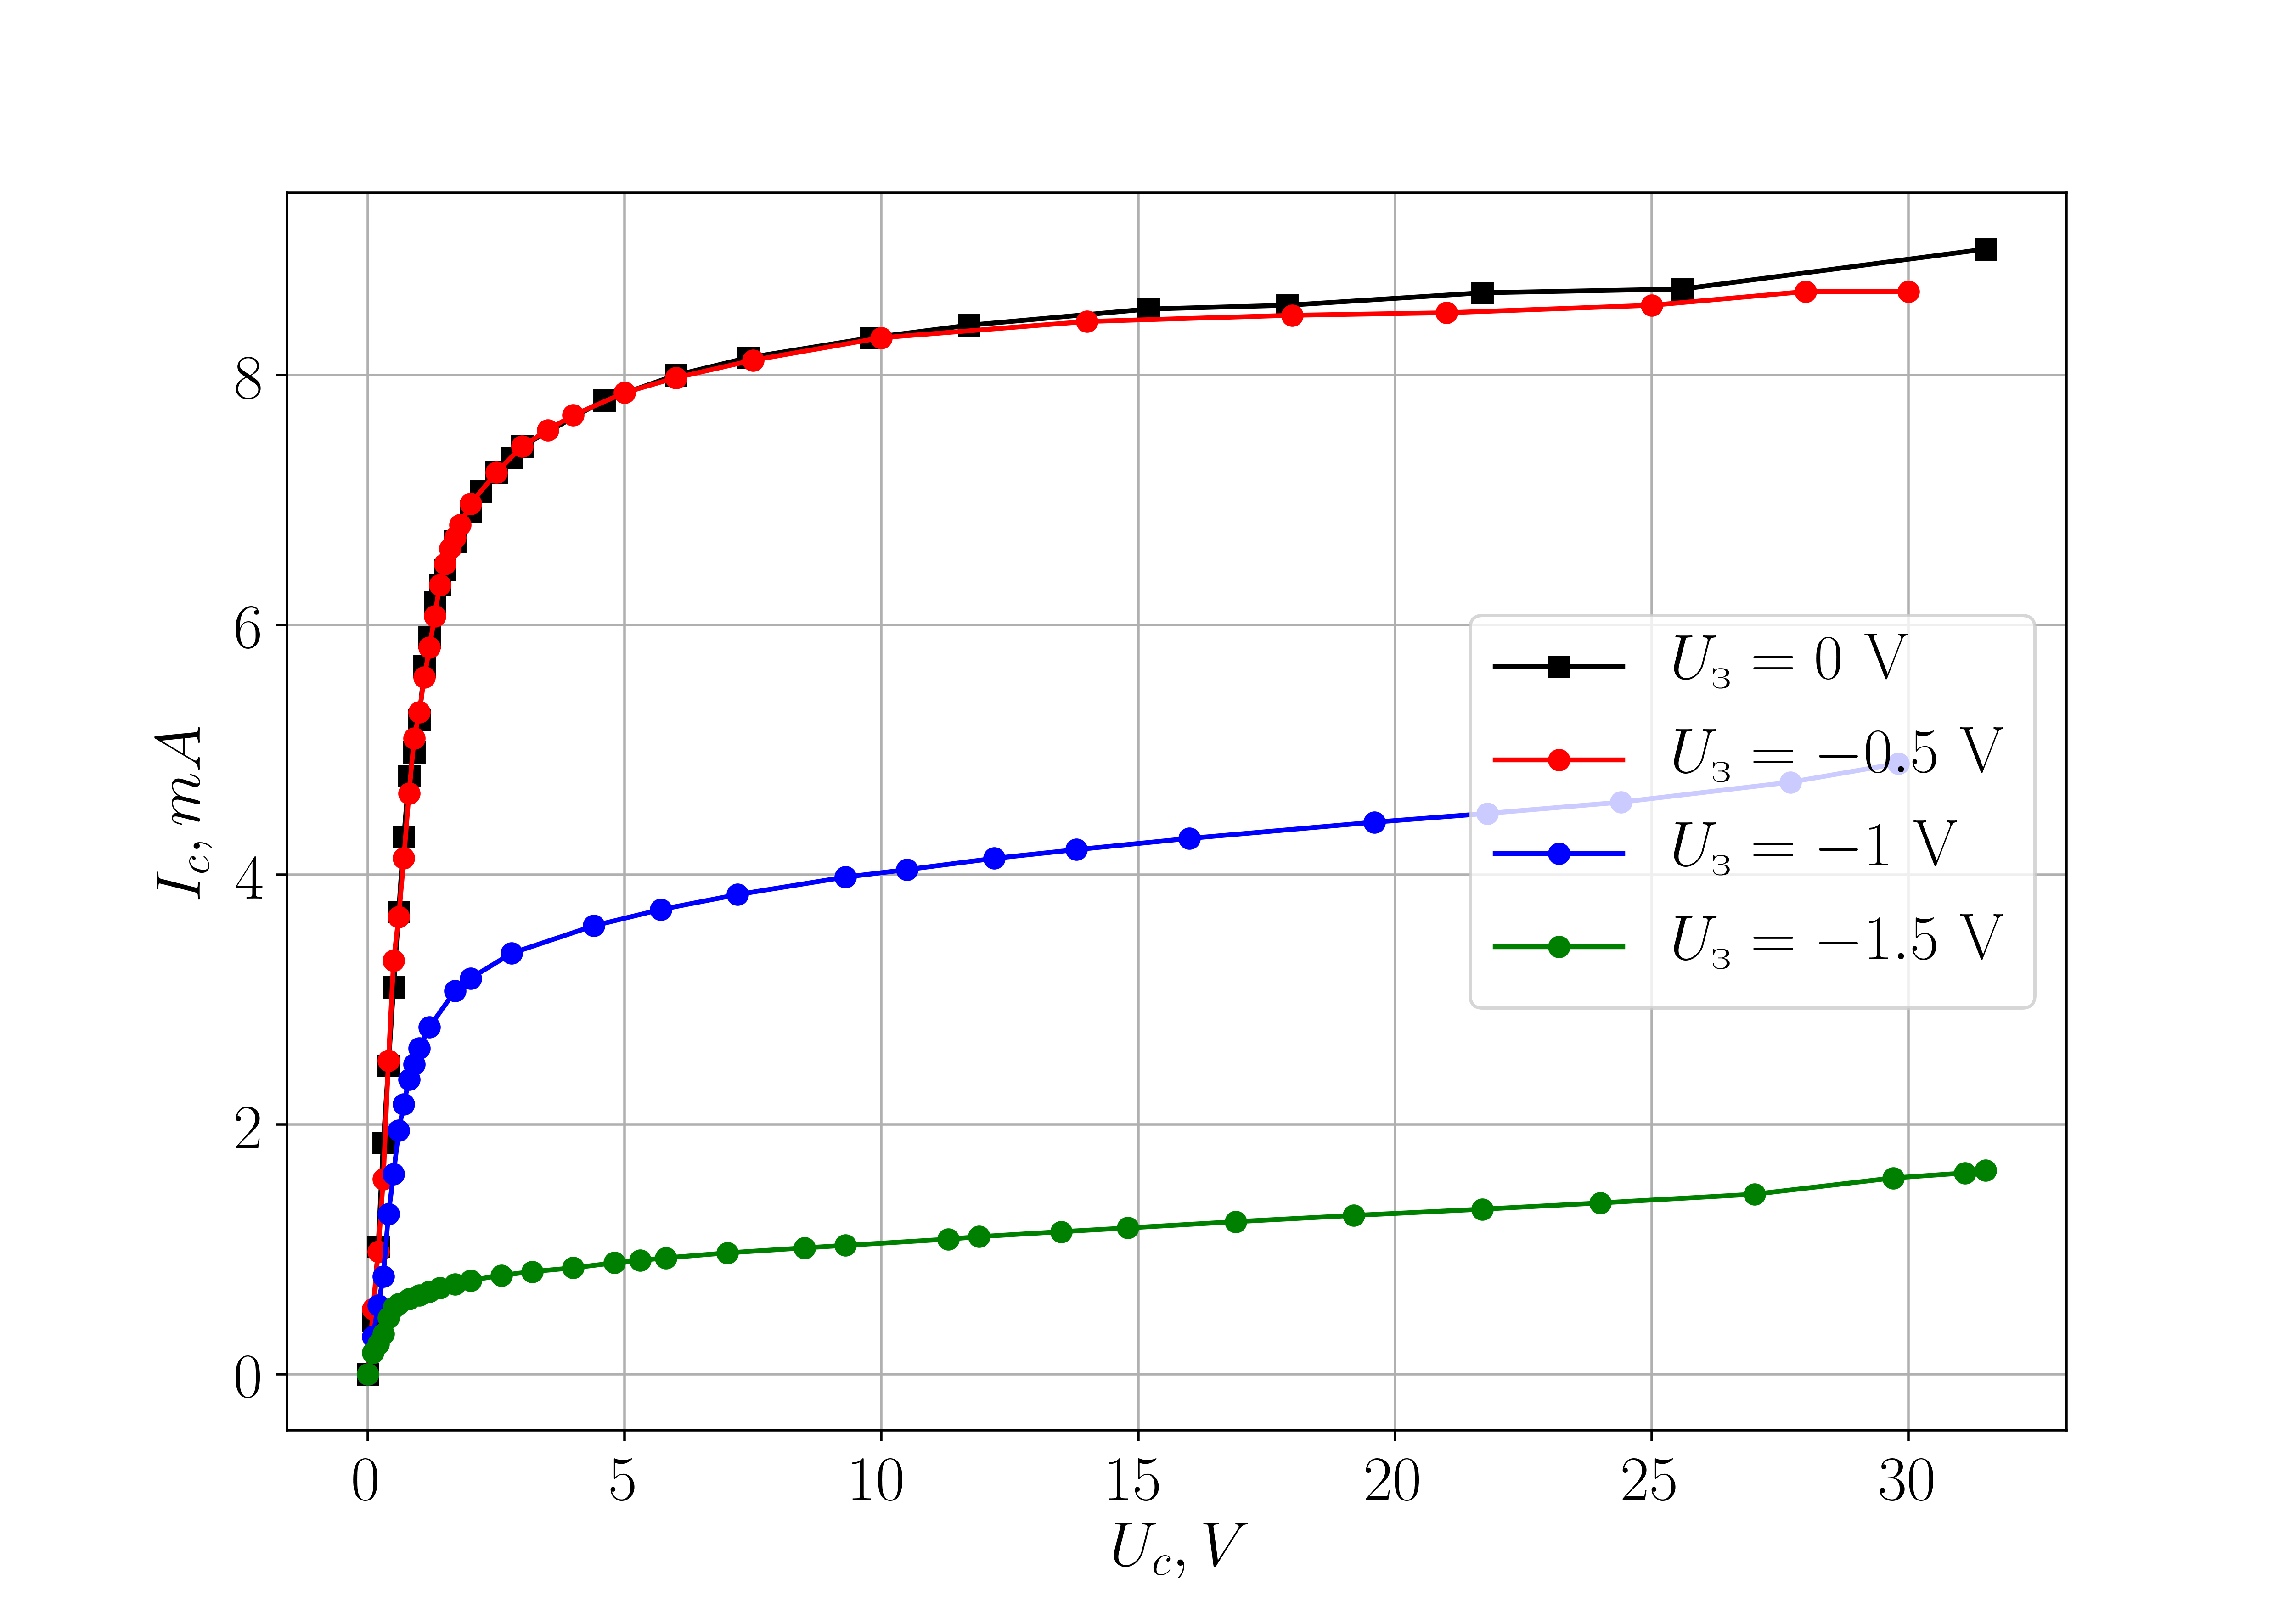
\includegraphics[width=0.7\linewidth]{fig/task2.png}
	\caption{Выходные характеристики транзистора для различных значений $U_{\text{з}}$??}
	\label{fig:8}
\end{figure}

\subsection{Исследование режима работы транзистора}
Для проведения исследования измерительный модуль был подключен к осциллографу и генератору сигналов по схеме на рис. \ref{fig:9}

\begin{figure}[h!]
	\centering
	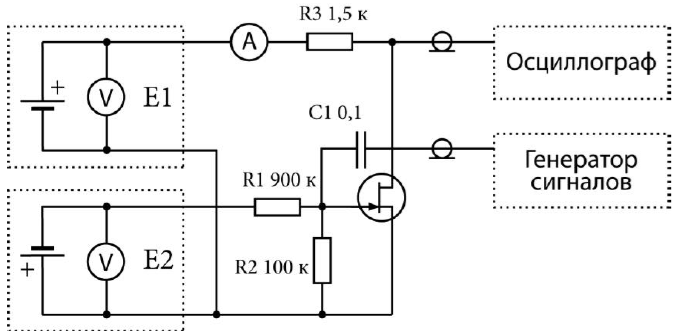
\includegraphics[width=0.5\linewidth]{imgs/ex3.png}
	\caption{Схема подключения для исследования режима работы транзистора}
	\label{fig:9}
\end{figure}
При выставленном напряжении $E_1 = 10$ В, с генератора сигналов подавался гармонический сигнал на амплитуде $\sim 200$
мВ и частоте $\sim 10$ кГц. Изменяя напряжние на затворе транзистора (регулируя $E_2$), транзистор был переведен в
следующие режимы: 
\begin{itemize}
	\item Отсечка - $E_2 = 20.3$ В, $I_c = 0$ мА??
	\item Насыщение - $E_2 = 8.8$ В, $I_c = 4.47$ мА
	\item Линейный - ??
\end{itemize}
Зафиксированные осциллограммы выходного сигнала приведены на рис. \ref{fig:10}
\begin{figure}[h!]
	\centering
	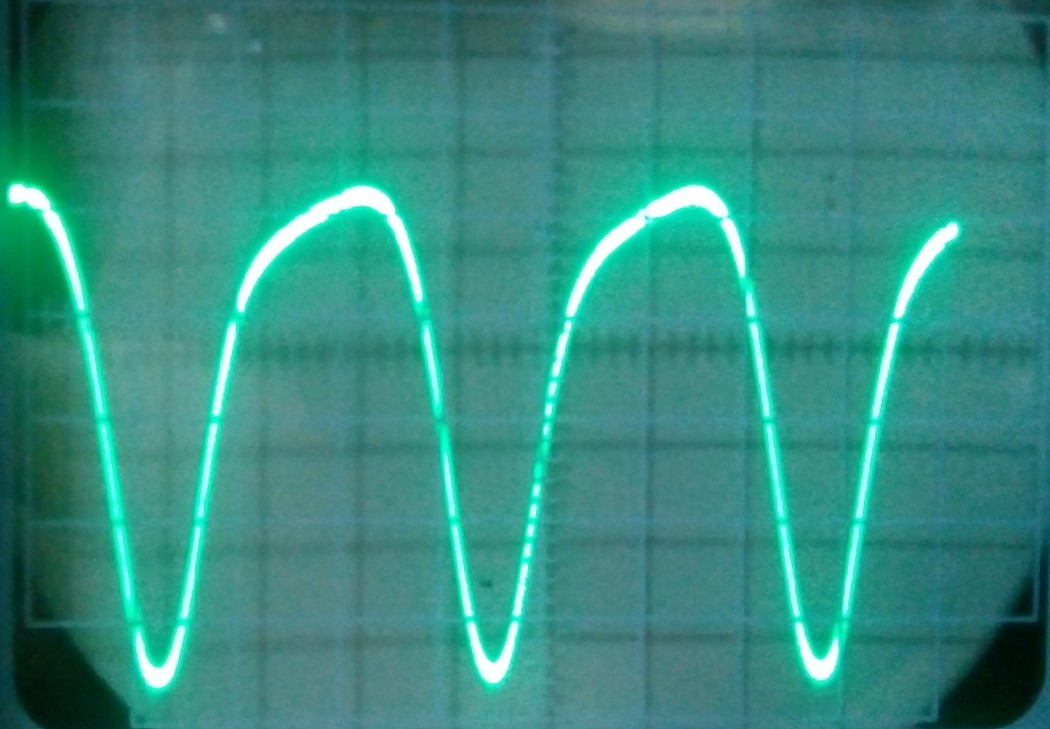
\includegraphics[width=0.3\linewidth]{imgs/1.jpg}
	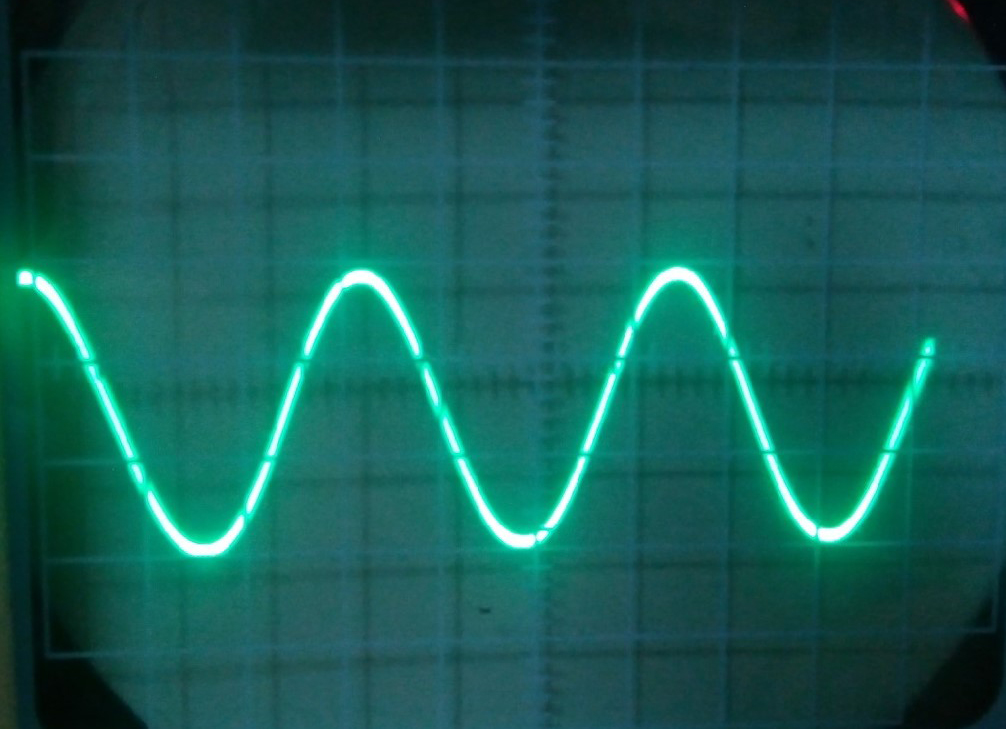
\includegraphics[width=0.3\linewidth]{imgs/2.jpg}
	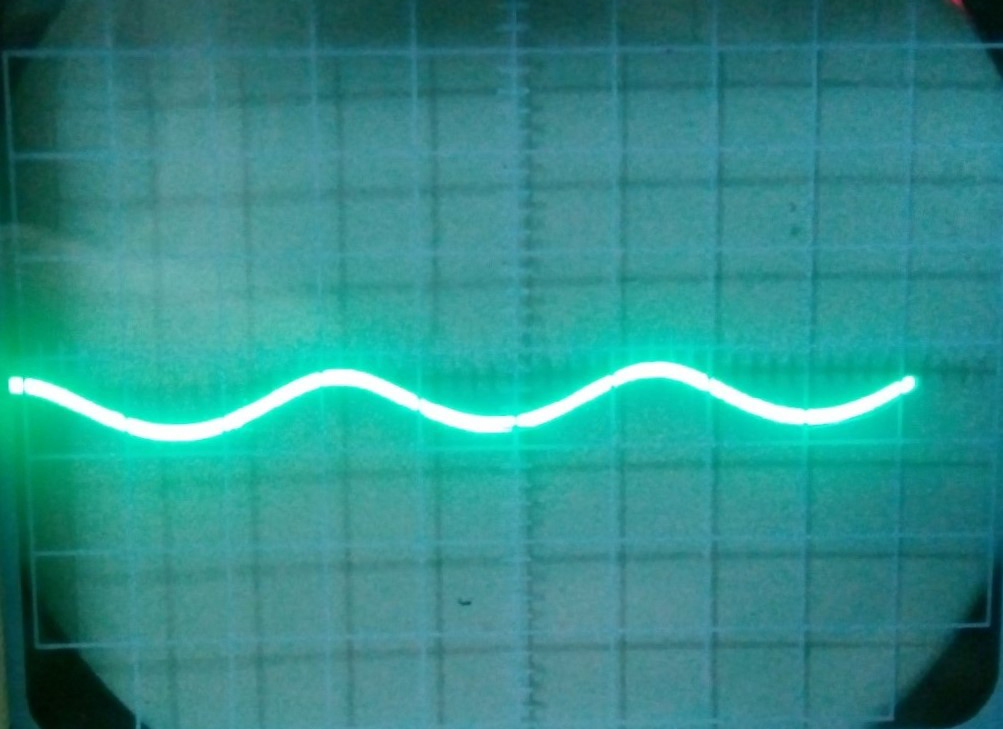
\includegraphics[width=0.3\linewidth]{imgs/3.jpg}
	\caption{Осциллограммы выходного сигнала для различных режимов работы транзистора??.}
	\label{fig:10}
\end{figure}

\subsection{Измерение коэффициента усиления усилителя}
Не изменяя схему подключения транзистора (см рис. \ref{fig:9}) было произведено измерение коэффициента усиления по напряжению.
При $E_1 = 10$ В, $U_{\text{з}} = 0.8$ В, $I_c = 5$ мА, и $U_{\text{ист}} = 200$ мВ была снята зависимость
выходного напряжения от частоты усиливаемого чигнала, по которой был рассчитан коэффициент усиления $K(f) =
U_{amp}/U_{\text{ист}}$ (см. рис.\ref{fig:11}).

\begin{figure}[h!]
	\centering
	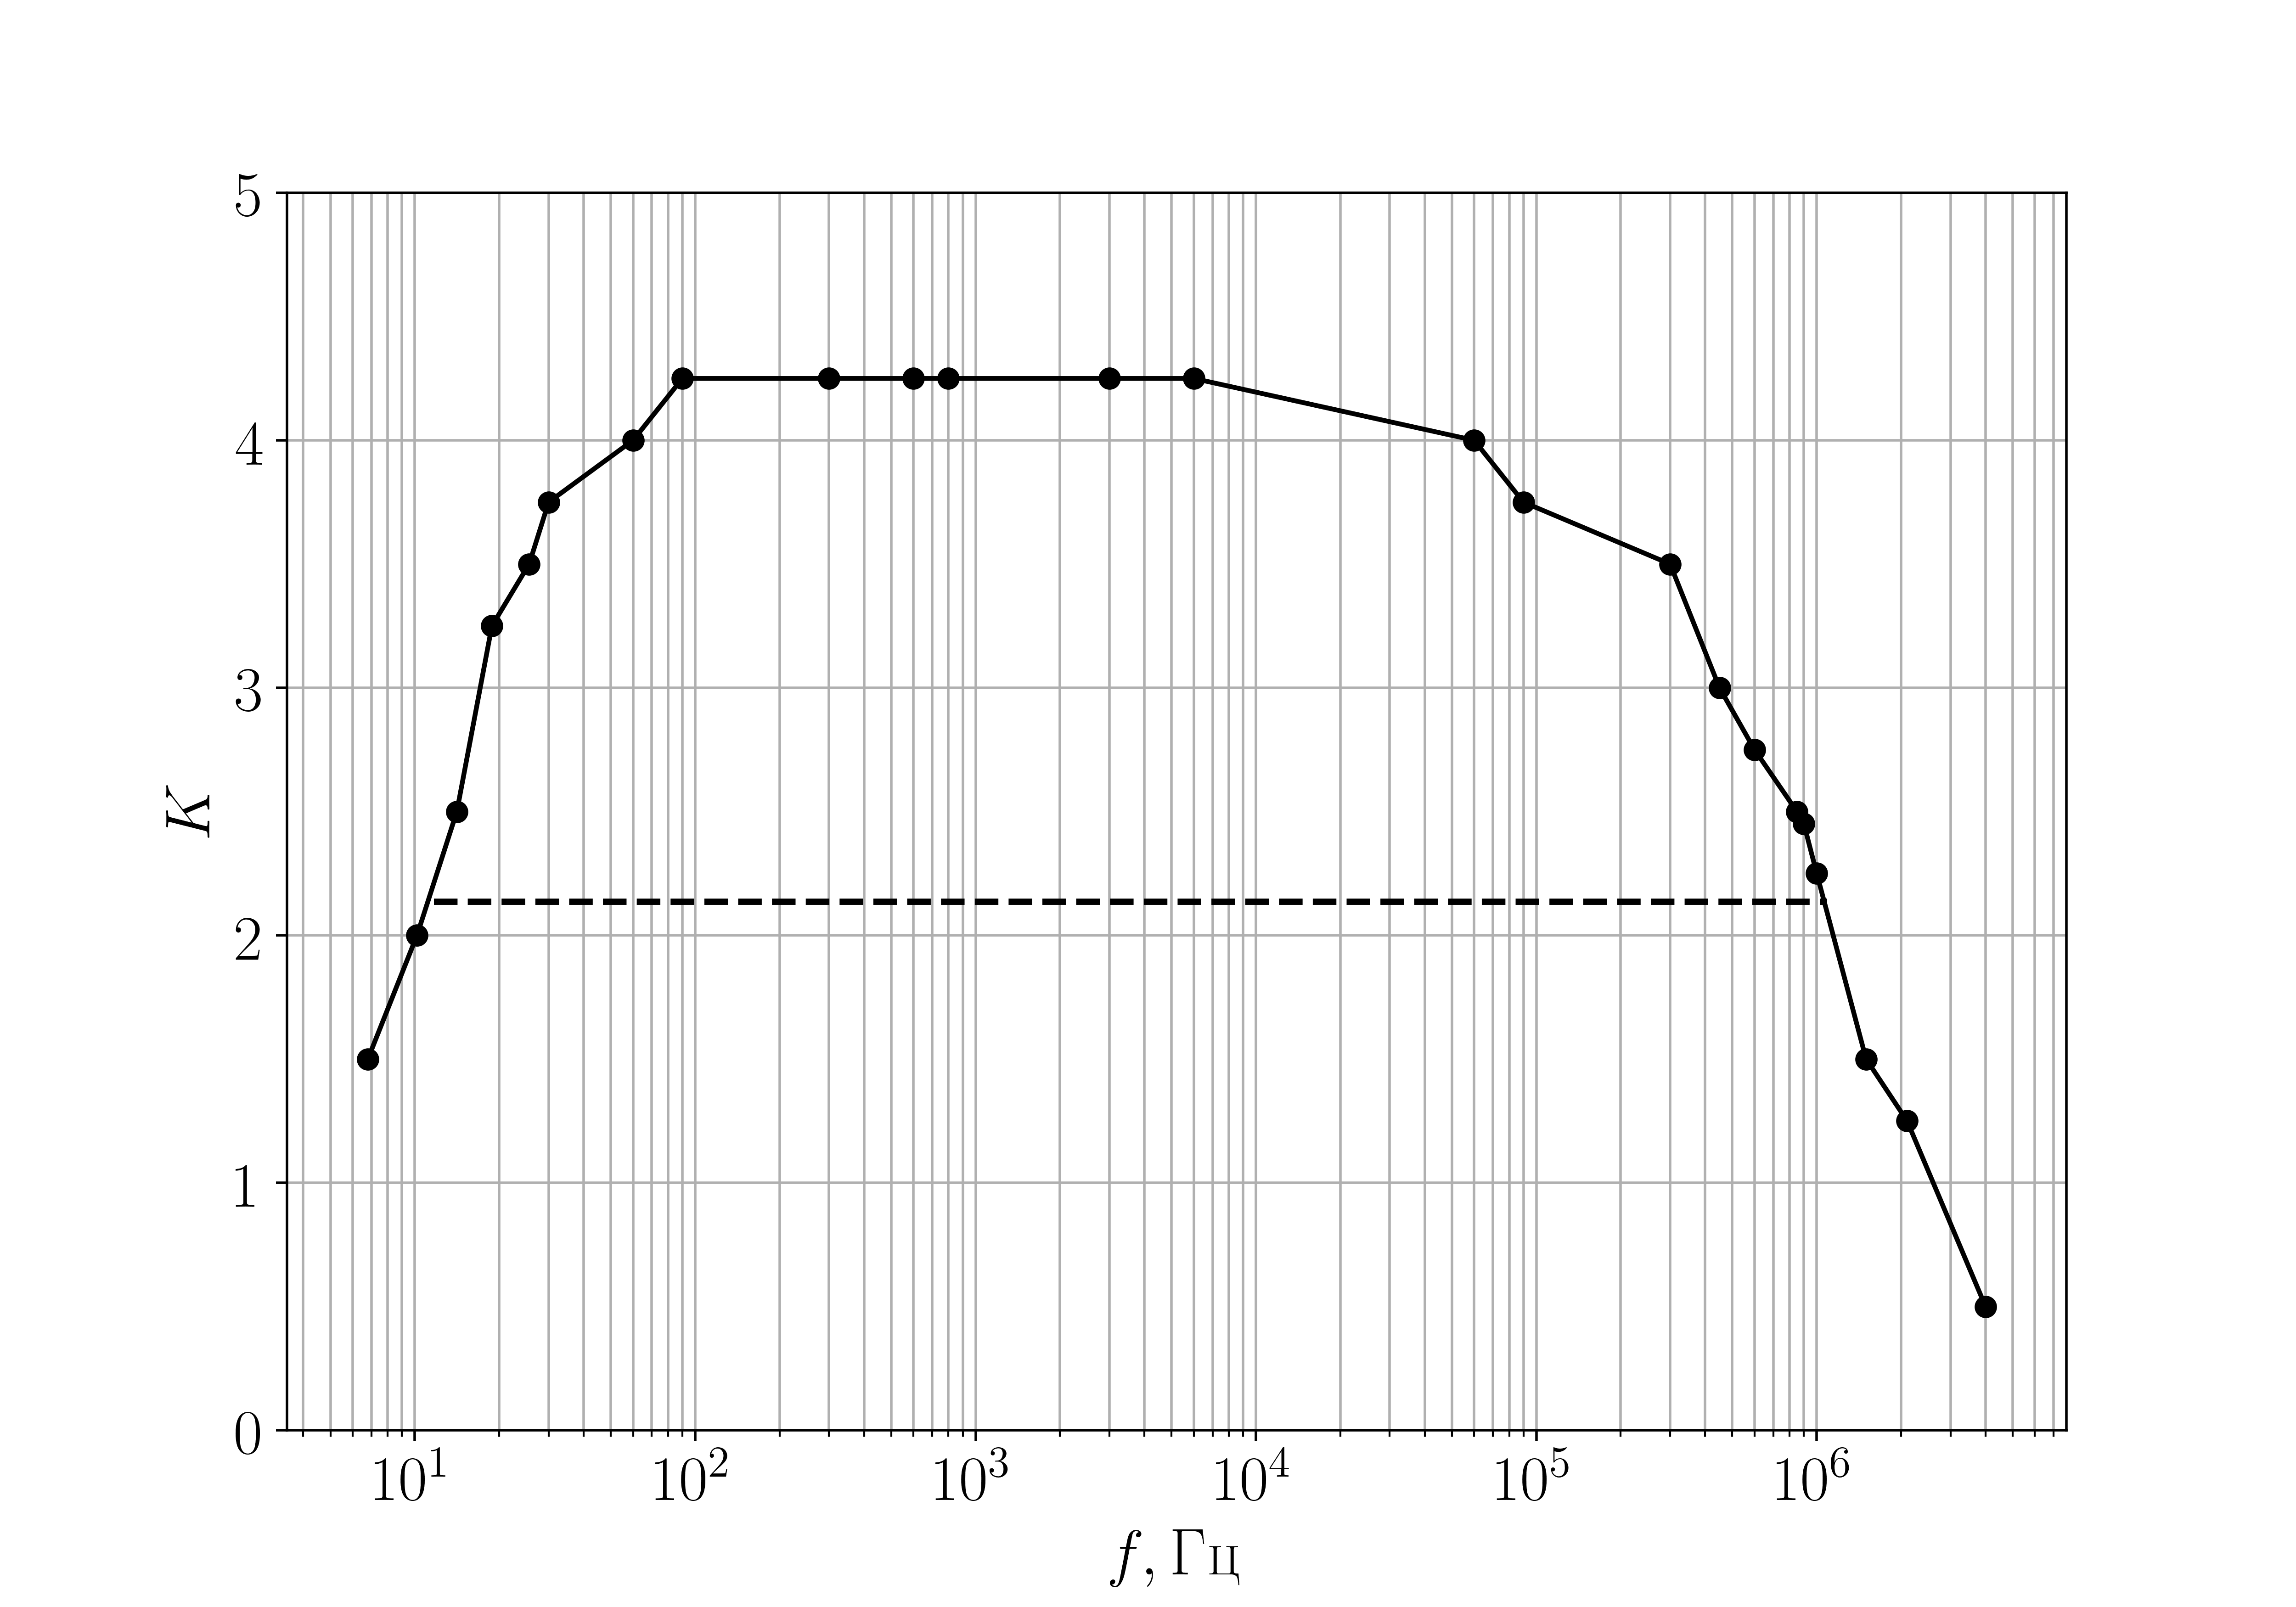
\includegraphics[width=0.8\linewidth]{fig/task4.png}
	\caption{Коэффициент усиления транзистора}
	\label{fig:11}
\end{figure}
Были определены предельные частоты усилителя - $f_1 = 12$ Гц, и $f_2 = 1$ МГц.

\subsection{Измерение времени переключения транзистора}
Транзистор был переведен в режим отсечки ($E_1 = 10$ В, $I_c = 3.3$ мА, $U_{\text{ист}} = 5.6$ мВ??). Для
определения времени переключения, с генератора подавался "меандр" на частоте $f = 120$ кГц с амплитудой $??$.

Определялось время переключения из режима отсечки в режим насыщения $t_1$, и время переключения из режима насыщения в
режим отсечки $t_2$. Результаты приведены на рис. \ref{fig:12}.
\begin{figure}[h!]
	\centering
	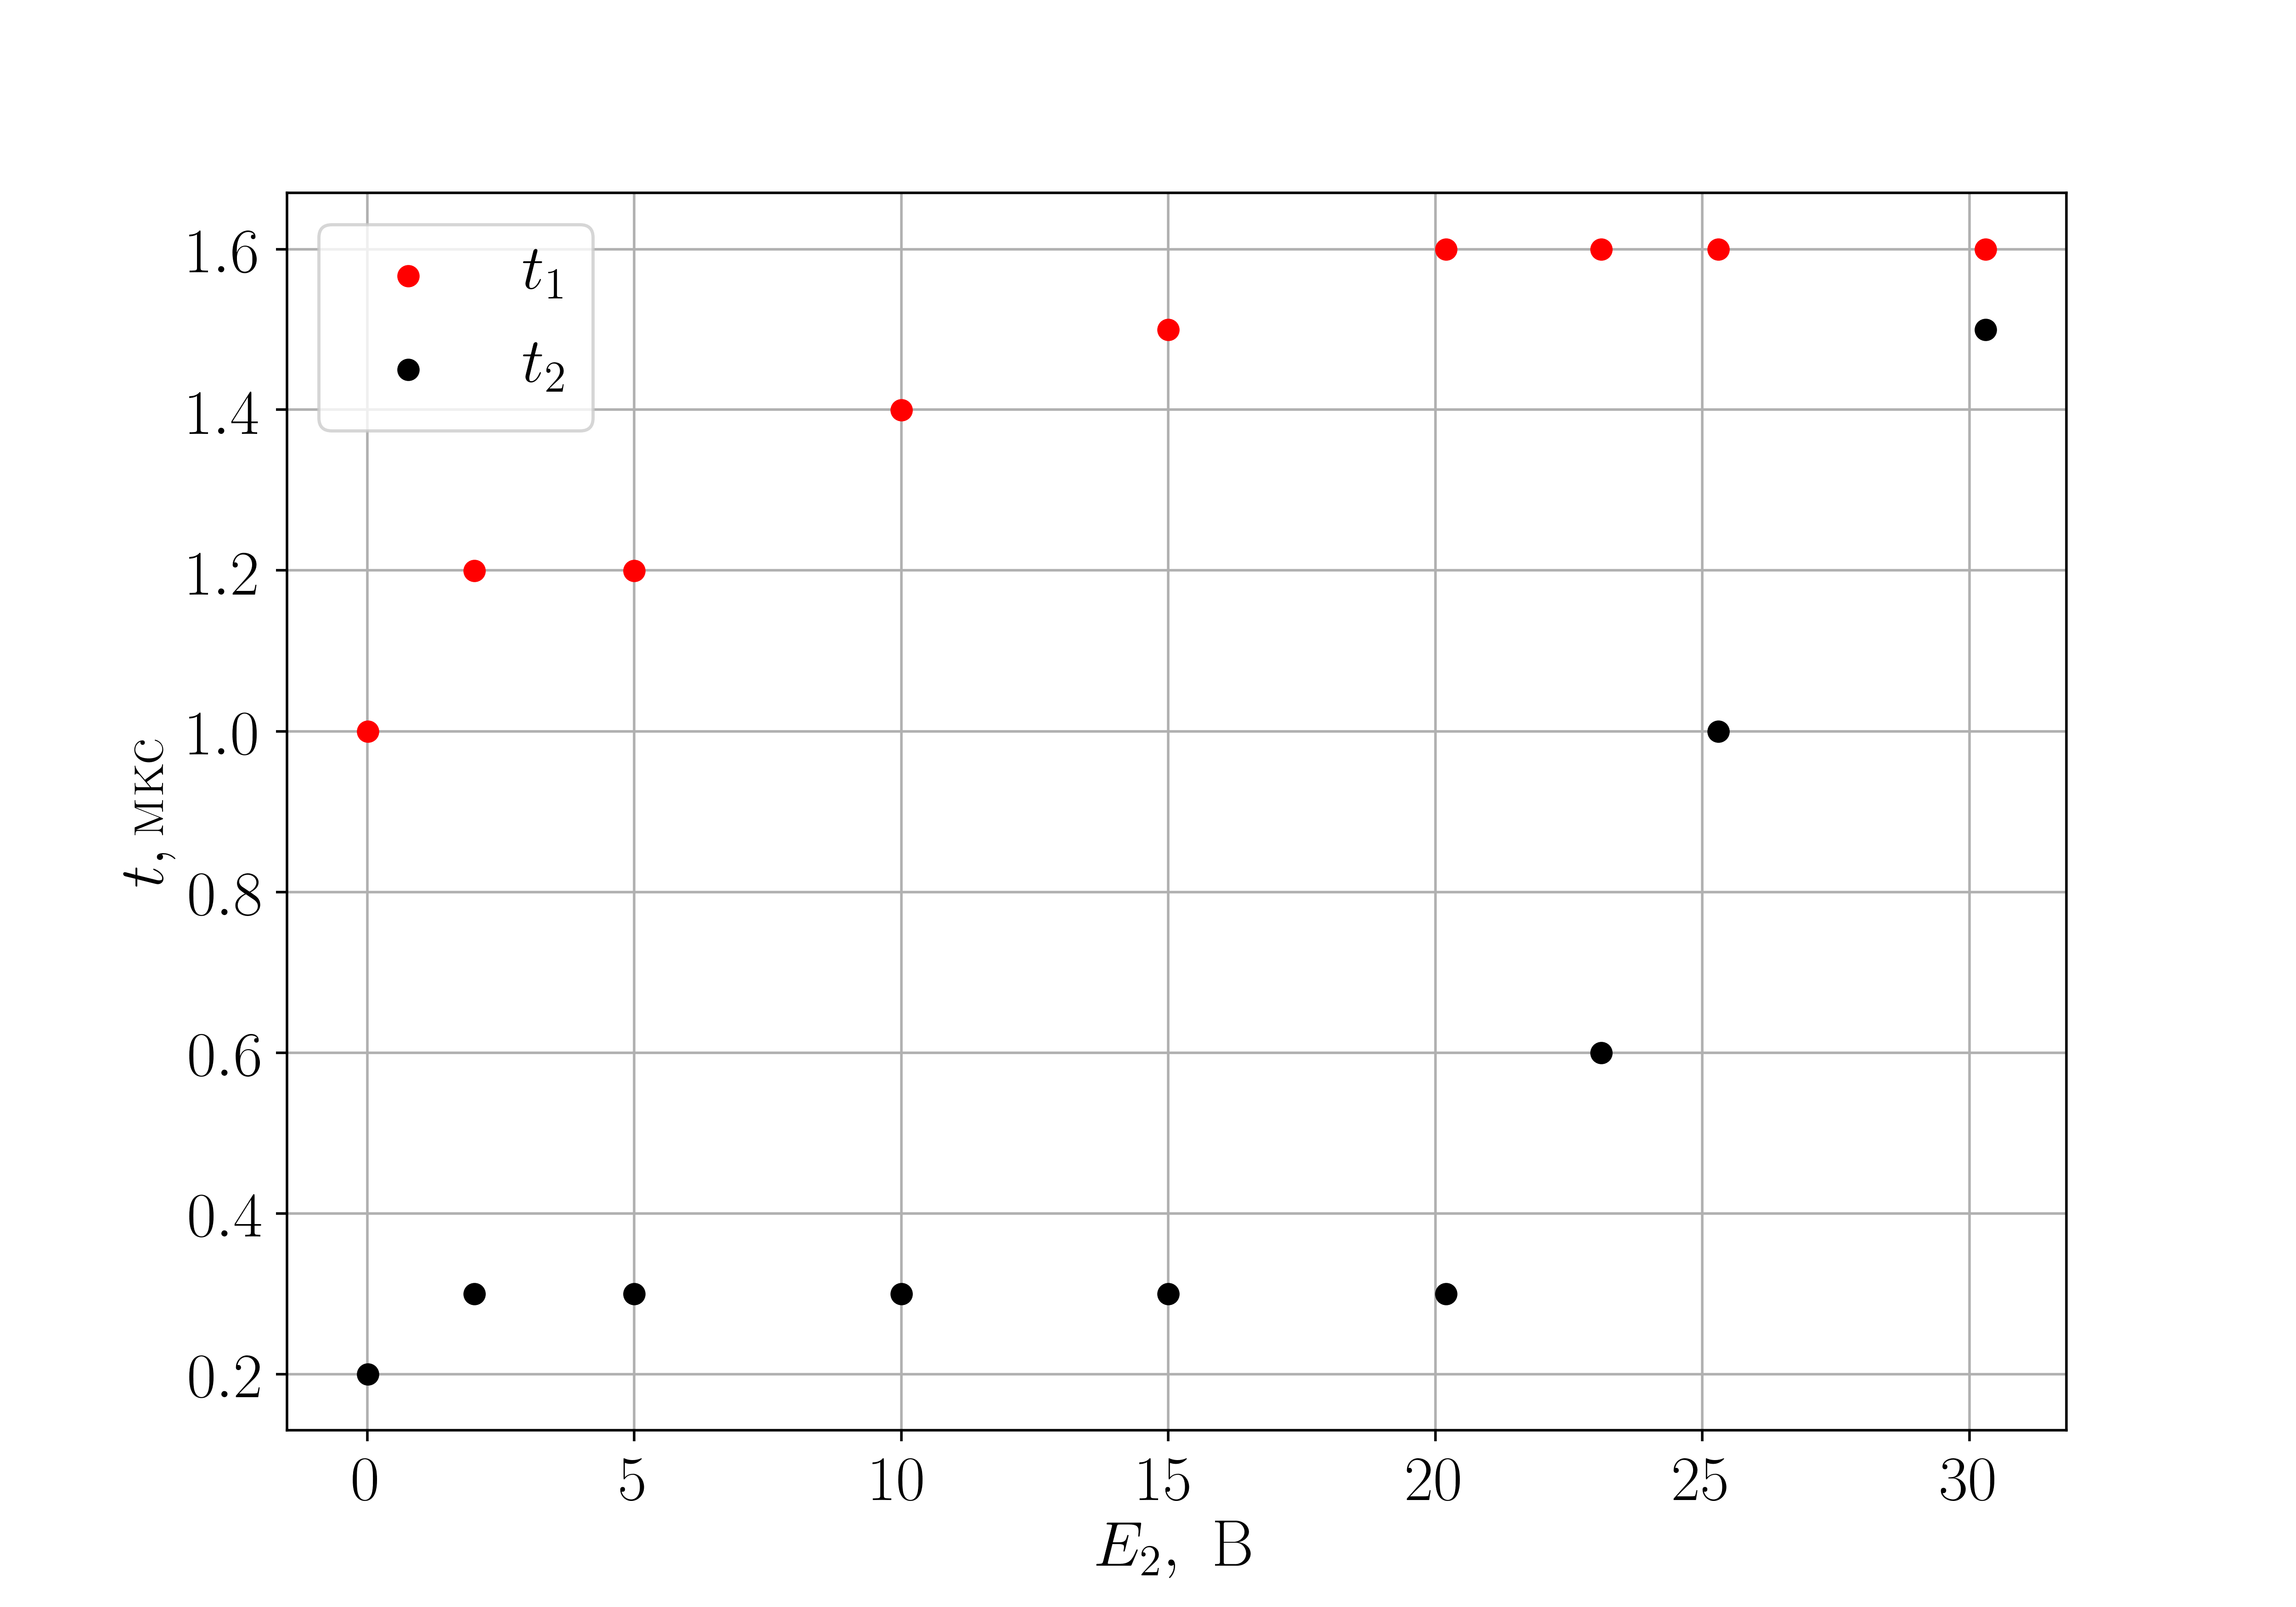
\includegraphics[width=0.8\linewidth]{fig/task6.png}
	\caption{Время переключения транзистора}
	\label{fig:12}
\end{figure}

\end{document}
